\documentclass[../main.tex]{subfiles}

\begin{document}

\section{Generación de la red \G{h} }

La generación de la red \G(h) no afecta en mayor medida la distribución de grado de los usuarios que participaron en la tendencia. 

\begin{figure}[h!]
    \centering
    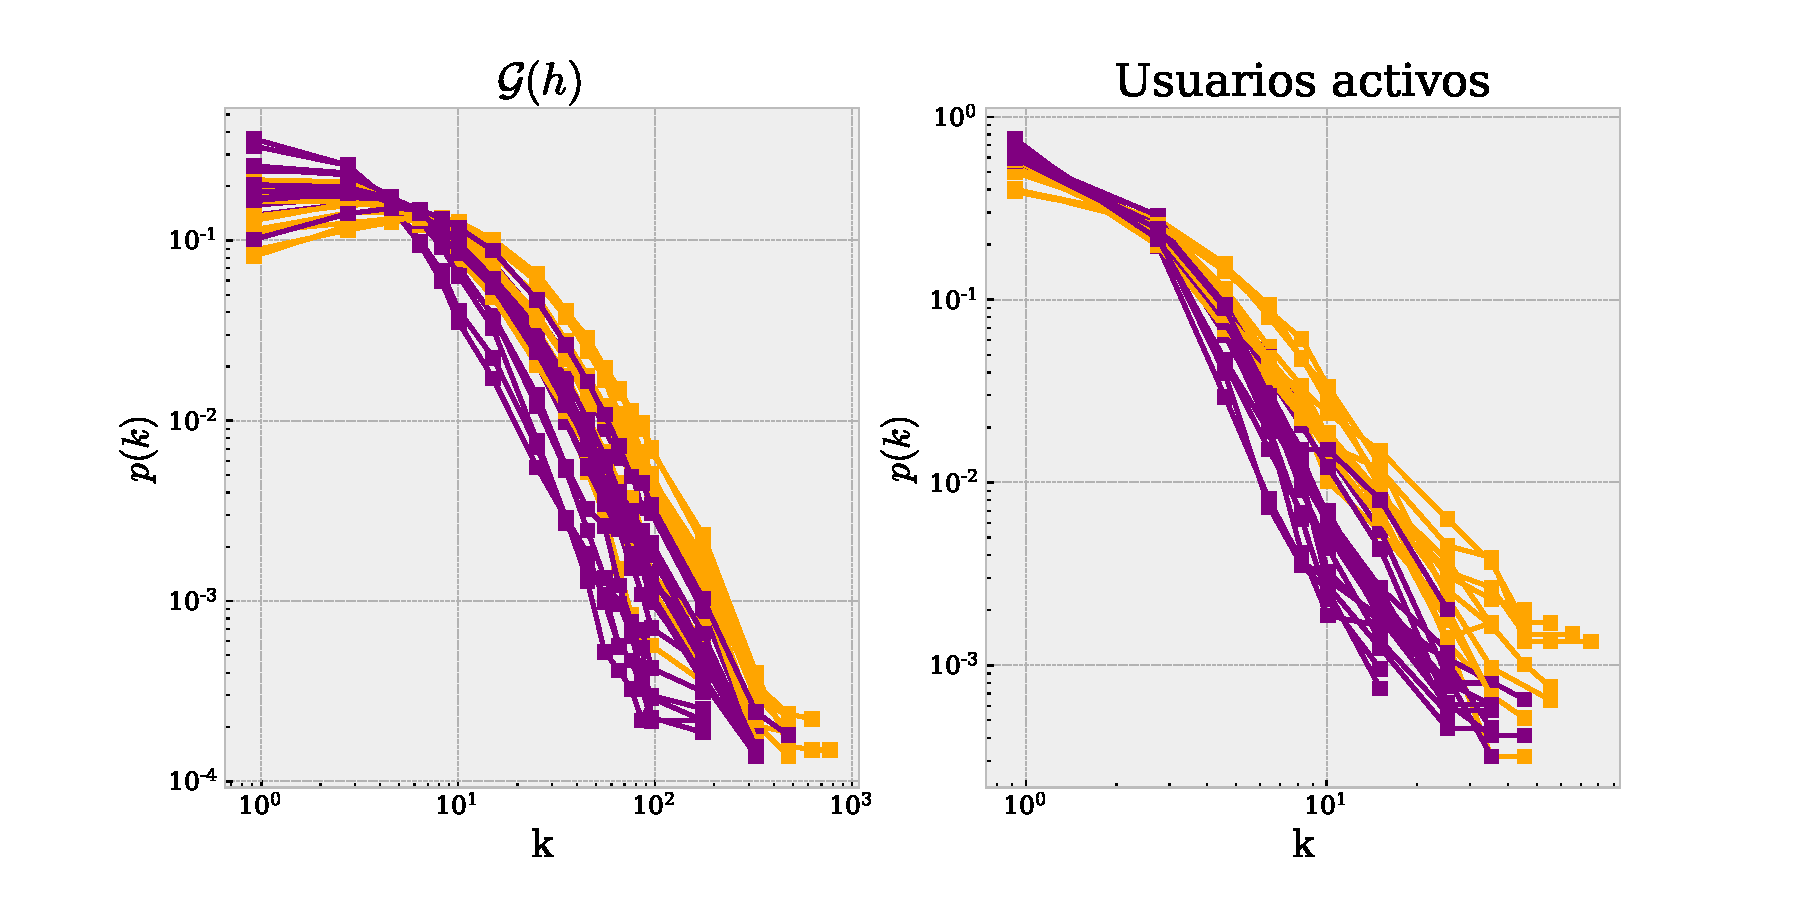
\includegraphics[scale = 0.5]{images/anexo_differencesNetworks.pdf}
    \caption{Caption}
    \label{fig:my_label}
\end{figure}


\end{document}

% Se reacciona al comportamiento de las personas maas no de la gente.




\begin{figure}
    \centering
    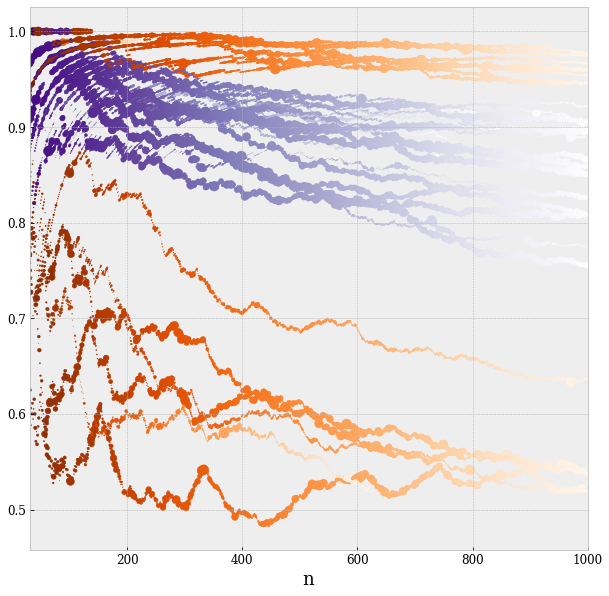
\includegraphics[scale = 0.5]{images/resultados_razonusuarios.png}
    \caption{ Comparativo de tendencias por los primeros 1000 \textit{Tweets}. Razón de usuarios nuevos en cada \textit{tweet} de los 1000 \textit{tweets} antes del periodo $t^{*}$. La líneas de color morado corresponden a tendencias con comportamiento explosivo.  } 
    \label{fig:resultados_1000Tweets}
\end{figure}